
\chapter{Grundlagen}

In diesem Kapitel beschäftigen wir uns zunächst mit der Installation und Konfiguration unserer Entwicklungsumgebung, in der wir später programmieren. Leider ist dies ein etwas aufwendiger Prozess und Sie müssen ihn jedes Mal durchgehen, wenn Sie einen neuen Rechner bekommen, oder fatalerweise Ihr Betriebssystem neu installierten. Auch Updates führen manchmal dazu, dass man Teile oder auch den gesamten Prozess neu durch gehen muss. Aber dazu später mehr.

\section{JDK und JRE}

Die Programmiersprache Java\footnote{Oracle and Java are registered trademarks of Oracle and/or its affiliates. Other names may be trademarks of their respective owners. Dies nur als rechtlicher Hinweis.} wurde 1991 bis 1992 von Patrick Naughton, Mike Sheridan, James Gosling und Bill Joy entwickelt (siehe \cite{wikijava}), damals noch bei Sun Microsystems. 2010 wurde Sun von Oracle gekauft. Nun ist Oracle -- nachdem noch weitere Firmen aufgekauft wurden -- im "`Besitz"' der Java Technologie. \index{Java}\index{Gosling, James}\index{Joy, Bill}\index{Sheridan, Mike}\index{Naughton, Patrick}

Java wird in zwei Versionen angeboten. Zum einen dem Java Runtime Environment (JRE). Dieses dient nur zum Ausführen von Java Programmen. Man kann mit dem JRE keine Programme schreiben. Das Programmieren ist mit dem Java Development Kit (JDK) möglich. Zudem enthält das JDK ein vollständiges JRE zur Ausführung der geschriebenen Programme. Das heißt: Ein JDK ist auch ein JRE, aber nicht umgekehrt. \index{JDK}\index{JRE}

Zudem bekommen Sie das JDK und JRE in 32-Bit oder 64-Bit Versionen. Falls Sie nicht einen älteren Prozessor oder sehr wenig Hauptspeicher besitzen, würde ich immer zu den 64-Bit Versionen tendieren. Ich habe zwar keine Untersuchungen darüber angestellt oder gelesen, aber subjektiv habe ich den Eindruck, dass die 64-Bit Java VM schneller ist. Daher empfehle ich diese.

Über die bekannte Seite 

\begin{Verbatim}[fontsize=\small]
https://www.java.com/de/
\end{Verbatim} 
erhalten Sie nur ein JRE. Damit können Sie nicht programmieren. Sie müssen auf folgende Seite gehen:
\begin{Verbatim}[fontsize=\small]
http://www.oracle.com/technetwork/java/javase/downloads/index.html
\end{Verbatim}
oder einfach auf 
\begin{Verbatim}[fontsize=\small]
http://download.oracle.com
\end{Verbatim}
und klicken sich dann zum JDK durch. Falls Sie schon einmal den Begriff Software Development Kit (SDK) gehört haben, so ist das JDK die Java Version eines solchen. 

Sie werden auf der Oracle Seite die Unterscheidung zwischen Standard Edition (JavaSE) und Enterprise Edition (JavaEE) finden. Man würde vermuten, das diese sich nur in der kommerziellen Ausrichtung unterscheiden. Tatsächlich sind dies aber unterschiedliche Technologien. Wir verwenden hier ausschließlich die Standard Edition, \textbf{nicht} die Enterprise Edition. Achten Sie bitte beim Download auf diese Unterscheidung!

Wenn Sie es heruntergeladen und installiert haben, sollten Sie in der Lage sein den folgenden Befehl in der Shell auszuführen:
\begin{Verbatim}[fontsize=\small]
C:>java -version
java version "1.8.0"
Java(TM) SE Runtime Environment (build 1.8.0-b128)
Java HotSpot(TM) 64-Bit Server VM (build 25.0-b69, mixed mode)
\end{Verbatim}

Sollten Sie obige Meldung nicht bekommen, dann müssen Sie Ihre Umgebungsvariablen anpassen, sodass das java.exe Executable gefunden werden kann.

\section{Virtual Machine}

Eine der zentralen Anforderungen an die Java Sprache war von Anfang an, dass die darin entwickelten Programme auf diversen Plattformen ohne Änderung lauffähig sein sollten. 
\begin{quote}
Write once, run anywhere!
\end{quote}
galt als Devise -- von Sun Microsystems. 

Um dieses Ziel zu erreichen, wurde eine Abstraktionsschicht in die Sprache eingebaut. Wie andere Compiler-Sprachen auch, übersetzt ein Java Compiler die von Menschen erzeugten Programme in einen maschinenlesbaren Code. Sprachen wie C, C++, Fortran, usw. erzeugen am Ende einen Code, der auf der Maschine, auf der der Compiler ausgeführt wurde, sehr gut und schnell läuft. Nicht so Java, der vom Java Compiler erzeugte Maschinen Code (Bytecode genannt) ist nur von einem anderen Programm lesbar. Dieses andere Programm liest den Java Bytecode und übersetzt die Bytecode Befehle direkt in Befehle des ausführenden Computers. Das bedeutet, dass dieses ausführende Programm die technischen Besonderheiten des Computers kennen muss, das Java Programm aber nicht mehr. Hat man nun auf verschiedenen Systemen ein solches Programm, das Java Bytecode lesen und ausführen kann, ist die Anforderung erfüllt, dass Java Programme einmal geschrieben und kompiliert werden müssen, dann aber auf allen Computern lauffähig sind, auf denen ein solches Programm, das Java Bytecode lesen und ausführen kann, installiert ist. 

Das "`Programm, das Java Bytecode lesen und ausführen kann"', wird als Java Virtual Machine\index{Virtual Machine}\index{Java Virtual Machine}\index{JVM} bezeichnet. Sie simuliert auf den verschiedensten Systemen, auf denen sie verfügbar ist, immer die selbe, nicht real existierende\footnote{Nicht real existierend, aber auf eine gewisse Weise wirkend, ist im Prinzip die Definition des Begriffs "`Virtualität"'. Der Grund, warum für eine bestimmte Plattform entwickelte Programme 'schnell' und 'effizient' ausgeführt werden, liegt daran, dass die Maschinenbefehle direkt auf den eingesetzten Prozessor abgestimmt sind und von diesem in kürzest möglicher Zeit ausführbar sind. Die Java Virtual Machine geht in ihrer Konzeption davon aus, dass bestimmte Maschinenbefehle auf allen Prozessoren zur Verfügung stehen. Sie muss also lediglich die Maschinenbefehle der Virtual Machine auf Maschinenbefehle des eingesetzten Prozessors übersetzen -- so die Theorie.}, Computerumgebung. Für diese Computerumgebung -- die Virutal Machine -- werden Java Programme entwickelt. 

Aktuell steht die Java Virtual Machine auf den Betriebssystemen Windows, Linux und MacOS zur Verfügung. Sowie von IBM eine spezielle Java Virtual Machine sowohl für Windows als auch AIX. Es gab früher mal eine Virtual Machine von Hewlett Packard im HP-UX Umfeld. Ich kann leider nicht sagen, was daraus geworden ist, da ich mit HP-UX nichts mehr zu tun habe. Es ist aber zu erwähnen, dass die Entwicklung einer Java Virtual Machine (JVM) eine recht aufwändige Sache ist und sich daher nur in sehr speziellen Fällen lohnt. Dies musste auch die Apache Foundation einsehen, die mit dem Apache Harmony Projekt eine offene, kostenlose und frei verfügbare Java Virtual Machine schreiben wollte. Im November 2011 wurde entschieden, das Projekt wieder einzustellen. Was -- unter anderem -- dem Umstand geschuldet war, dass mit OpenJDK nach dem Kauf von Sun durch Oracle eine Open Source Implementierung einer JVM verfügbar war. OpenJDK enthält den Source Code der ehemaligen Sun JVM, aus dem die kommerziellen und/oder patentrechtlich geschützten Teile entfernt und durch offene Implementierungen ersetzt wurden. OpenJDK ist vor allem im Linux Bereich die bevorzugte JVM.

Zusätzlich ist es möglich, direkt Bytecode zu schreiben, den eine Virtual Machine ausführt. Dies machen sich andere Sprachen zu nutze, z.B. Scala. Der Scala Compiler übersetzt Scala Programme in den Bytecode der Java Virtual Machine, welche dann die Scala Programme genauso ausführt, wie Java Programme. 

\section{Compiler}

Der zu Java gehörende Compiler heißt \texttt{javac}\index{javac}. Machen wir mal ein kleines Experiment. Erzeugen Sie ein Verzeichnis und legen dort eine Datei an mit dem Namen \texttt{Test.java}. Öffnen Sie diese Datei in einem Editor und schreiben Sie folgenden Text hinein:

\begin{lstlisting}
public class Test {
  public static void main(String[] args) {
    System.out.println("Hello World!");
  }
}
\end{lstlisting}\label{code:test}\index{Hello World!}

Speichern Sie die Datei und schließen Sie sie. Öffnen Sie nun eine Kommandoshell in dem selben Verzeichnis und rufen Sie den Compiler auf mit 
\begin{Verbatim}
javac Test.java
\end{Verbatim}
Der Compiler wird wortlos die gewünschte Aktion durchführen. In Ihrem Verzeichnis sollte nun zusätzlich eine \texttt{Test.class} Datei erzeugt worden sein. Rufen Sie danach 
\begin{Verbatim}
java Test
\end{Verbatim}
auf, es sollte ein "`Hello World!"' erscheinen. Glückwunsch: Ihr erstes -- so hoffe ich -- Java Programm.

Der Aufruf des "`java"' Programms vor Ihrem "`Test"' Programm ist der Aufruf der JVM. Die JVM ist die java.exe, die dann Ihr Programm im Bytecode ausführt. Sie haben damit ein "`Hello World!"' Programm geschrieben, dass sowohl auf Windows, Linux als auch MacOS lauffähig ist. Ist doch gar nicht so schlecht, oder?

Wir werden es hierbei schon mit Informationen über den Compiler belassen. Wir kommen später noch einmal darauf zurück. 

\section{IDE}

Üblicherweise programmiert und kompiliert man nicht mit einfachen Editoren und einer Shell. Sie können es, gar keine Frage. Aber angenehm ist das nicht. 

Zur Entwicklung bedient man sich meistens besonderer Programme, die das Entwickeln von Software einfacher machen. Sogenannte Integrated Development Environments (IDE). \index{IDE}\index{Integrated Development Environment}

Im Java Umfeld gibt es diverse IDE's, hier sei nur auf die bekanntesten und gleichzeitig kostenlosen hingewiesen. 

\begin{enumerate}
\item Eclipse (\texttt{http://www.eclipse.org})\index{Eclipse}
\item Netbeans (\texttt{http://www.netbeans.org})
\item IDEA IntelliJ Community Edition (\texttt{http://www.jetbrains.com})
\end{enumerate}
Von Jetbrains\index{Jetbrains} gibt es auch eine kommerzielle Version ihrer IDEA IntelliJ Umgebung, die Community Edition ist aber kostenlos.

Wir werden uns hier auf die Netbeans IDE\index{Netbeans} beschränken. Das hat zum einen den Grund, dass alle Funktionalitäten der Netbeans IDE kostenlos sind. Das gilt zwar auch für Eclipse, aber seit dem Upgrade auf die Version 4.0 habe ich persönlich die Freunde an Eclipse verloren. Das verschiedene Gründe, die ich auf Rücksicht und Respekt vor der vielen Arbeit der Eclipse Entwickler, für mich behalte. Sagen wir einfach, ich hätte eine Münze geworfen.

Ich möchte Sie hier an dieser Stelle ermutigen, sich alle Entwicklungsumgebungen einmal zu installieren und genau auszuprobieren. Vielleicht gefällt Ihnen ja eine andere besser und Sie kommen gut damit zurecht. Jede hat ihre Stärken und Schwächen. Ich selbst verwende oft verschiedene IDE's für verschiedene Zwecke.

\subsection{Installation}
Der Installer von Netbeans\footnote{Wir verwenden hier die Netbeans Version 8.0} ist schnell herunter geladen und zum Setup brauchen Sie im allgemeinen keine zusätzlichen Informationen. Die Einstellungen sollten auf den Vorgabe Werten belassen werden. Sofern Sie bereits ein JDK installiert haben, wird Netbeans dies automatisch finden. Sollte es hier Schwierigkeiten geben, oder Sie erst später das JDK installiert haben, müssen Sie folgende Einstellung vornehmen:

Suchen Sie im Netbeans Installationsverzeichnis die netbeans.conf Datei
\begin{Verbatim}
C:\Program Files\NetBeans 8.0\etc\netbeans.conf
\end{Verbatim}
Dort sollten Sie die Angabe
\begin{Verbatim}
netbeans_jdkhome="C:\Program Files\Java\jdk1.8.0"
\end{Verbatim}
finden. Sollte diese Angabe falsch sein, oder nicht zu Ihrem JDK passen, sollten Sie diese Einstellung anpassen.
Ich bin hier davon ausgegangen, dass Sie ein 64-Bit JDK und die 64-Bit Version von Netbeans installiert haben. Diese beiden müssen zueinander passen. Haben Sie das 32-Bit JDK installiert, müssen Sie auch die 32-Bit Version von Netbeans installieren. Sonst bekommen Sie Schwierigkeiten.

Wenn Sie Netbeans zum ersten Mal starten, bekommen Sie die Start Page angezeigt. Sie erscheint im Editor Fenster und kann durch das kleine Kreuz am Namensreiter geschlossen werden. Ist diese geschlossen, haben Sie einen Blick auf die leere IDE. 

\subsection{Projekte}

Alle IDE's arbeiten in sogenannten Projekten.\index{Projekt} Sie können sich ein Projekt als ein Verzeichnis mit darin enthaltenen Dateien vorstellen. Nicht nur Ihre Java Dateien werden darin liegen, sondern auch alle Projekt-spezifischen Einstellungen der IDE. Abbildung \ref{nb:newproj} zeigt den Wizard, mit dem man ein neues Projekt anlegen kann. Klicken Sie auf "`next"', wählen Sie den Haken ab, eine "`Main-Klasse"' zu erzeugen und geben Sie dem Projekt einen Namen, zum Beispiel "`TestApplication"'.

\begin{figure}[h]
\centering
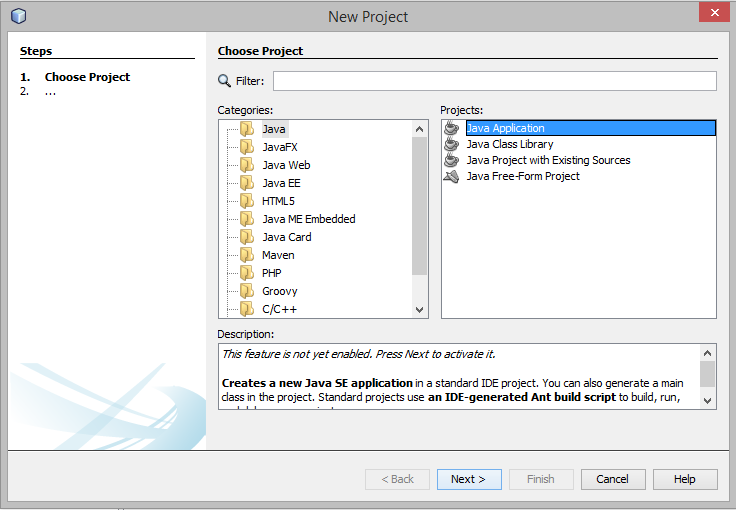
\includegraphics[width=\textwidth]{img/nb001}
\caption{Wizard zur Erzeugung eines neuen Java Projekts}
\label{nb:newproj}
\end{figure}

Wenn Sie das Projekt angelegt haben, sollte Ihr Projekt so wie in Abbildung \ref{nb:emptproj} aussehen.

\begin{figure}[h]
\centering
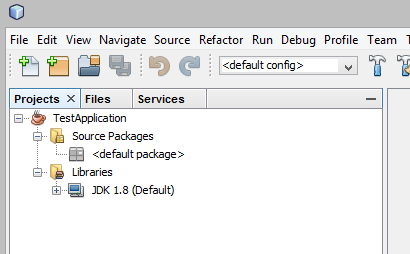
\includegraphics[]{img/nb002}
\caption{Leeres, neues Java Projekt}
\label{nb:emptproj}
\end{figure}

\newpage
Wenn Sie auf den "`Source Package"' Order mit der rechten Maustaste klicken, erscheint das Kontext Menü. Wählen Sie "`New $\rightarrow$ Java Class ..."' und füllen Sie den Wizard so aus, wie in Abbildung \ref{nb:newclass}.

\begin{figure}[h]
\centering
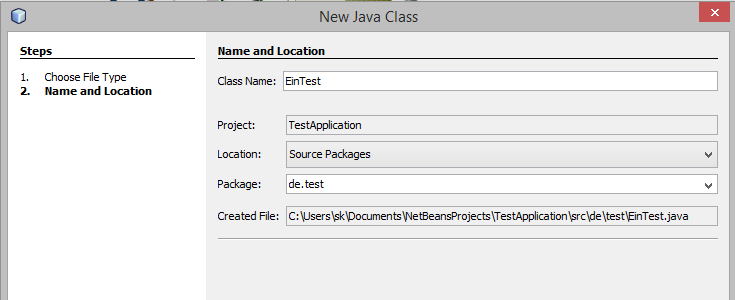
\includegraphics[width=\textwidth]{img/nb003}
\caption{Neue Klasse}
\label{nb:newclass}
\end{figure}

Danach sollte in Ihrem Editor ein Fester auf gehen, mit dem folgendem Inhalt 

\begin{lstlisting}
/*
 * To change this license header, choose License Headers in Project Properties.
 * To change this template file, choose Tools | Templates
 * and open the template in the editor.
 */
package de.test;
/**
 *
 * @author kesper
 */
public class EinTest {
    
}
\end{lstlisting}
Die Zeilen, die mit den *-Zeichen beginnen, sind Kommentare. In Java (und auch anderen Sprachen) sind Kommentare Informationen für den Entwickler, sie werden vom Compiler grundsätzlich ignoriert. Es gibt zwei Arten von Kommentaren, nämlich den einzeiligen und den begrenzten Kommentar. \index{Kommentar}

Einzeilige Kommentare beginnen mit zwei Slash-Zeichen "`//"'. Sie können an jeder beliebigen Stelle im Source Code auftauchen und gelten immer bis zum Ende der Zeile. Das heißt, alles in einer Zeile, das hinter zwei Slash-Zeichen steht, ist ein Kommentar, auch wenn Sie nach dem Kommentar noch Code einfügen wollen, geht das nicht, es wird auch weiterhin als Kommentar betrachtet. 

Der begrenzte Kommentar hat Start- und Stopp-Symbole. Slash Stern(\texttt{/*}) öffnet einen Kommentar und Stern Slash (\texttt{*/}) schließt ihn wieder. Auch wenn es sich bei dem Kommentar nur um ein Wort handelt, können Sie nach einem begrenzten Kommentar -- selbst in der selben Zeile -- weiterschreiben. Sollten Sie einen längeren Kommentar einfügen wollen, lohnt sich der begrenzte Kommentar immer. 

Kommentare werden Ihnen am Anfang unsinnig erscheinen. Wenn Sie aber eine Weile programmieren und ältere Code Stücke analysieren möchten, werden Sie für Kommentare -- sofern sie beschreiben, was Sie sich beim Erzeugen des Codes gedacht hatten -- sehr dankbar sein.

In Java haben bestimmte Kommentare noch eine weitere Funktion: Sie dienen der Dokumentation Ihres Codes. Solche Kommentare, die mit "`/**"' Slash-Doppelstern beginnen, gehören zum sogenannten Javadoc\index{Javadoc} System. Dies ist eine recht elegante Art, wie Sie innerhalb Ihres Source Codes Kommentare schreiben und diese automatisiert zu einer HTML Dokumentation zusammen fügen lassen können. Dies wird später noch genauer erklärt.  

\subsection{Packages}\label{sect:package}
Als nächstes fällt auf, dass am Anfang des Codes eine Paket Anweisung steht. Packages (dt. Pakete)\index{Package}\index{Paket} sind Ansammlungen von Klassen. Es ist zwar möglich Klassen ohne Package zu erzeugen, das hatten wir mit der Test Klasse in Kapitel \ref{code:test} so gemacht, aber dies stellt eine schlechte Angewohnheit dar. Warum, werden wir im Folgenden sehen. Aus unserem Code Pakete zu schnüren hat zwei grundlegende Motivationen: 

\begin{description}
\item[Füge zusammen, was zusammen gehört]
Wenn sich verschiedene Klassen mit dem selben oder Variationen des selben Themas beschäftigen, ist es sinnvoll diese in ein Paket zusammen zu stellen. Alleine der Ordnung willen. Suchen Sie dann eine Klasse, finden Sie sie dort, wo sie sie vermuten könnten, nämlich dort wo alles liegt, was zu dem Thema gehört. 
\item[Bibliothekten]
Wenn Sie später einmal sogenannte Bibliotheken schreiben, also Code Teile, die Sie nicht in verschiedenen Projekten neu entwickeln, sondern wiederverwenden möchten, ist es sehr viel einfacher Kollisionen zu verhindern, in dem Sie Packages verwenden. Genauso ist es einfacher alle Klassen, die zu einem Package gehören in eine Bibliothek zusammenzuführen, wenn man sie anhand ihres Paketes identifizieren kann. 
\end{description}

Packages sind ein Ordnungsprinzip und gleichzeitig trennen sie sogenannte Namensräume. Sie können zwei oder mehr Klassen mit dem selben Namen haben, wenn diese in verschiedenen Paketen liegen. Nicht das Sie dies tun sollten, aber Sie \textit{könnten}, wenn Sie verschiedene Pakete verwenden.

Ein Paket besteht aus einem einfachen, frei wählbaren Namen. Es dürfen allerdings keine Sonder- oder Leerzeichen enthalten sein, sowie darf keine Zahl am Anfang des Paketnamens stehen. Pakete haben eine Hierarchie, das bedeutet, dass es Pakete in anderen Paketen gibt. Dies wird so dargestellt, dass ein Punkt zwischen Eltern Paket und aktuellem Paket geschrieben wird. In unserem Beispiel haben wir das oberste Paket mit "`de"' bezeichnet, so wie es von Sun einmal empfohlen wurde. Danach kommt unser Paket test, in dem wir unsere Klasse angelegt haben. Die sogenannte Signatur unseres Paketes ist also "`de.test"'. 

Die Standard Bibliothek von Java enthält viele nützliche Klassen. Diese sind alle in ihre eigenen Pakte und Unter-Pakete einsortiert. Sie beginnen mit "`java."' bzw. "`javax."'. Sie können keine eigenen Pakete erzeugen, die mit "`java."' oder "`javax."' beginnen. Dies verhindert der Compiler, weil diese Pakete reserviert sind.

\section{Aufgaben}
\begin{enumerate}
\item Was ist der Unterschied zwischen einem JDK und einem JRE?
\item Was ist eine Virtual Machine?
\item Wofür steht die Abkürzung IDE?
\item Was ist ein Package?
\end{enumerate}

